\documentclass{article}
\usepackage{verbatim,fancyvrb}
\usepackage{pifont}
%\usepackage[authoryear]{natbib}
\usepackage[pdftex]{graphicx}
\usepackage{gretl}
\usepackage[hyphens]{url}
\usepackage{hyperref}
\usepackage[letterpaper,body={6.3in,9.15in},top=.8in,left=1.1in]{geometry}

\setlength{\parindent}{0pt}
\setlength{\parskip}{1ex}
\setlength{\abovecaptionskip}{0pt}

\newcommand{\startappendices}{%
\newcounter{appcount}
\setcounter{appcount}{0}
 \renewcommand{\thesection}{Appendix \Alph{appcount}}}

\newcommand{\myappendix}[1]{%
\addtocounter{appcount}{1}
\section{#1}}

\newenvironment{funcdoc}
{\noindent\hrulefill\\[-10pt]}
{\medskip}

\title{geoplot: cartography in gretl}
\author{Allin Cottrell and Jack Lucchetti}

\begin{document}

\maketitle

\textbf{Notice}: As of this writing the \textsf{geoplot} package is
work in progress. You are welcome to try it but expect some bugs and
do not bank on the user interface remaining unchanged. We should also
mention a non-temporary peculiarity of \textsf{geoplot}. We have found
it preferable to implement its core functionality via built-in
functions, coded in C. For basic usage, therefore, it's not necessary
to load the package explicitly via ``\texttt{include geoplot.gfn}'',
as one would usually expect.

That said, section~\ref{sec:prelim} below covers some preliminaries
which we hope will help the reader to understand what's going
on. Section~\ref{sec:workflow} describes the basic workflow for
producing a map image via gretl. Section~\ref{sec:example} then
provides a simple worked example and section~\ref{sec:pairing}
addresses a potential stumbling block. Section~\ref{sec:opts} goes
over the current options to the core \texttt{geoplot} function in
detail; section~\ref{sec:gui} tells you what's available via gretl's
graphical interface; section~\ref{sec:expert} explains some ``expert''
refinements; and section~\ref{sec:future} gives our current thinking
on possible future directions for maps in gretl.

\section{Preliminaries}
\label{sec:prelim}

Given gretl's user base and vocation, we assume that people will be
primarily interested in ``thematic'' maps, in which geographical areas
get different colors according to some variable of interest (for
example regions of a country are colored according to their
unemployment rates). Fancier maps are out of scope for the
present. From here on we'll simply refer to maps of this sort as
``maps'' and the geographical entities they contain (which may be
countries, states, counties, l\"ander or whatever) as
``regions''. Plotting a map typically involves drawing a number of
polygons, filled with appropriate colors, to some device (the screen,
or a file).\footnote{One may want to draw colored lines, such as
  rivers or roads: not for now.}

The essential ingredients for doing this are
\begin{enumerate}
   \item A geometrical description of the regions.
   \item The data for coloring the polygons.
   \item Appropriate software for producing the map.
\end{enumerate}

\subsection{The geometry}
\label{sec:geometry}

Let's say we have $n$ regions, indexed by $i$. Region $i$ is
represented geometrically as a collection of $k_i$ polygons (think
islands in an archipelago), indexed by $j$. Each polygon is defined by
$h_{i,j}$ coordinates. Typically, each coordinate vector has two
elements, latitude and longitude.\footnote{In some cases you may have
  a third element---altitude being the most obvious candidate---or
  more.  But we're not getting into that right now.}

The information on each region has two components:
\begin{description}
\item[Metadata] At minimum this should include the region's
  identifier(s), as strings and/or numerical codes. Other information,
  such as land area, may also be included. You can think of this as a
  dataset with $n$ observations and several variables, possibly
  string-valued.
\item[Polygons] A representation of the region's shape on the map, in
  the form of one or more polygons, each taking the form of an array
  of X--Y pairs, typically latitude and longitude. You can think of
  this as an array of arrays of 2-column matrices: the outer array is
  of size $n$; inner array $i$ contains $k_i$ matrices, each with two
  columns.
\end{description}

Several file formats can be used for storing the geometry
information.\footnote{The site
\url{https://ec.europa.eu/eurostat/web/gisco/geodata/reference-data/administrative-units-statistical-units/nuts}
offers a nice collection for European NUTS regions (NUTS =
Nomenclature of Territorial Units for Statistics).}
Gretl supports what are probably the two most common formats:
\begin{itemize}
\item GeoJSON files: plain JSON files with a pre-specified internal
  structure, regulated by RFC 7946. Basically, an array of regions (or
  ``features'') with each element containing the metadata and the
  polygons, under the \texttt{properties} and \texttt{geometry} keys,
  respectively.  This is our preferred format.
\item ESRI shapefiles: more of a ``legacy'' format, but still very
  common in the wild. These maps come as collections of several files,
  usually zipped together. The essential components are an
  \textsf{xBase} file, with \texttt{dbf} extension, holding the
  metadata; the shapefile proper with extension \texttt{shp}, holding
  the polygons; and an index file with extension \texttt{shx}, used
  to speed up operations when reading the data.
\end{itemize}

\subsection{The payload data}
\label{sec:payload}

By ``payload'' we mean the data used for coloring the regions.  We
assume that the payload is available as a gretl series. This typically
means that the user has a data file (in native \texttt{gdt} format or
some other format gretl can read) in which each line represents a
region, as illustrated in Table~\ref{tab:payload}. Note in particular
the ``id'' column.  We assume that the map metadata contain sufficient
information to establish a correspondence with the dataset containing
the payload: either a numerical code or a suitable string-valued
variable.  One thing one quickly learns in exploring a variety of
\texttt{geojson} and \texttt{shp} files is that there's no telling how
the regions will be ordered; one \textit{cannot} assume that they
occur in what one might think of as ``standard'' order (e.g.\
alphabetical order for US states).

\begin{table}[htbp]
\begin{center}
\begin{tabular}{llrr}
  %\hline
  id	& State & Pop2019 & Pop2010 \\
  \hline \\ [-1.75ex]
  1	& Alabama	& 4903185	& 4779736  \\
  2     & Alaska	& 731545	& 710231   \\
  101   & American Samoa	& 55641	& 55519	  \\
  3	& Arizona	& 6278717	& 6392017  \\
  4	& Arkansas	& 3017825	& 2915918  \\
  5	& California	& 39512223	& 37254523 \\
  6	& Colorado	& 5758736	& 5029196  \\
  7	& Connecticut	& 3565287	& 3574097  \\
                & \vdots & \\
  %\hline
\end{tabular}
\end{center}
\caption{Typical format for a payload dataset}
\label{tab:payload}
\end{table}


\subsection{The software backend}
\label{sec:software}

In principle one could represent maps using any one of the many
plotting libraries around, but gretl uses \textsf{gnuplot}, which we
already use for all other kinds of plot. Some insight into the
\textsf{gnuplot} commands we use can be gained from
Appendix~\ref{sec:gnuplot}.

Given the geometry data and the payload, writing a \textsf{gnuplot}
script for producing the map is straightforward. And in most cases
\textsf{gnuplot} can produce a plot in short order. You might have to
wait a little if there are many regions, of complex shapes,
represented in high precision in the source map file.

\section{The workflow}
\label{sec:workflow}

Typical workflow for producing a thematic map in gretl is likely to be
as follows.

\begin{enumerate}
\item You \cmd{open} the map-datafile as a gretl dataset; this reads
  in the metadata so gretl's \dollar{nobs} will be equal to the number
  of regions, $n$.
\item You add the payload data, via the \texttt{append} or
  \texttt{join} commands or in some other way.
\item You decide on some details of your map (appearance, format,
  etc.), with sensible defaults being available.
\item Finally, you create the map.
\end{enumerate}

Point 1 is handled by using the existing \texttt{open} command on the
map-datafile. The filename extensions recognized for this purpose are
\texttt{json} or \texttt{geojson} for GeoJSON files, \texttt{dbf} or
\texttt{shp} for ESRI shapefiles.\footnote{In principle we could read
  the polygons at this point and store them in RAM, but for now we
  don't. We just read in the metadata, but store the path to the
  associated geometry file internally.} Point 2 is also handled by
existing gretl commands.

As for points 3 and 4, these are handled by the new (built-in)
\texttt{geoplot} function, which has the following signature.
\begin{code}
function void geoplot(const string mapfile,
	              const series payload[null],
	              const bundle options[null])
\end{code}
Here \texttt{mapfile} is the (required) name of the file containing
the polygons, \texttt{payload} is the (optional) series with which to
colorize the polygons, and \texttt{options} is an (optional) bundle to
contain one or more elements governing the appearance or destination
of the plot.
\begin{itemize}
\item If the \cmd{geoplot} call follows on the opening of a map
  metadata file in the same session, you can give the accessor
  \dollar{mapfile} in place of an actual filename for the
  \texttt{mapfile} argument, since gretl already knows what file we're
  talking about.
\item If the \texttt{payload} argument is given as \texttt{null} or
  omitted then the map is drawn ``as is'', without any
  colorization. This can be useful if you just want to see what the
  polygons look like.
\item If the \texttt{options} bundle is omitted all options are set to
  their default values---which means, in short, that you see the map
  on screen but nothing is saved. For full details on the available
  options see section~\ref{sec:opts}.
\end{itemize}

\section{An example}
\label{sec:example}

For this example we'll produce a map showing GDP per capita of the six
founder countries of the EU, using three files: script
\texttt{founders.inp}, data file \texttt{founders.csv} and map
\texttt{founders.geojson}. In this case the required files are small
enough to be readily inspected by hand.  The content of
\texttt{founders.csv}, which holds what will be the payload, is shown
in Listing~\ref{tab:founders-csv}.

\begin{script}[htbp]
\begin{scode}
Name,code,pop,area,gdp
Belgium,BE,11365834,30528,534230
France,FR,67024633,632833,2833687
Germany,DE,82437641,357386,3874437
Italy,IT,61219113,301338,2147744
Luxembourg,LU,589370,2586.4,65683
Netherlands,NL,17220721,41543,880716
\end{scode}
\caption{Content of \texttt{founders.csv}}
\label{tab:founders-csv}
\end{script}

\begin{script}[htbp]
  \begin{scode}
{"type": "FeatureCollection", "features": [
 {"geometry": {"type": "Polygon", "coordinates": [[[40.40360,
     30.79039], [40.59686, 30.49366], [40.65087, 30.29746], ... ]]},
   "type": "Feature", "properties": {"CNTR_NAME": "Belgique",
     "ISO3_CODE": "BEL", "CNTR_ID": "BE", "NAME_ENGL": "Belgium",
     "FID": "BE"}, "id": "BE"},
 {"geometry": {"type": "MultiPolygon", "coordinates": [[[[40.18497,
     29.45664], [40.23634, 29.39875], [40.57754, 29.35021], ...],
     [[[42.66689, 20.70300], [42.57348, 20.41660], ...]]},
   "type": "Feature", "properties": {"CNTR_NAME": "France",
     "ISO3_CODE": "FRA", "CNTR_ID": "FR", "NAME_ENGL": "France",
     "FID": "FR"}, "id": "FR"},
  ...
\end{scode}
\caption{Excerpt of \texttt{founders.geojson}}
\label{tab:json-xrpt}
\end{script}

The JSON file is too big to show here in full but small enough to
examine in any text editor.\footnote{Even Microsoft's
  \texttt{Notepad}!} Listing~\ref{tab:json-xrpt} contains a
representative excerpt. Note that while Belgium is a single polygon
France is an array of polygons (``\texttt{MultiPolygon}''), because of
Corsica.

\begin{script}[htbp]
\begin{scode}
open founders.geojson --frompkg=geoplot

join founders.csv gdp pop --ikey=FID --okey=code
series gdppc = 1000*gdp/pop

opts = defbundle("plotfile", "GDPpc.plt", "inlined", 1)
geoplot($mapfile, gdppc, opts)
\end{scode}
  %$
\caption{Content of \texttt{founders.inp}}
\label{tab:founders-script}
\end{script}

The \texttt{founders.inp} script is shown in
Listing~\ref{tab:founders-script}, and what we get after opening the
\texttt{geojson} file in gretl is in Listing~\ref{tab:founders-meta}.

\begin{script}[htbp]
\begin{scode}
     CNTR_NAME    ISO3_CODE      CNTR_ID    NAME_ENGL          FID

1     Belgique          BEL           BE      Belgium           BE
2       France          FRA           FR       France           FR
3  Deutschland          DEU           DE      Germany           DE
4       Italia          ITA           IT        Italy           IT
5    Luxemburg          LUX           LU   Luxembourg           LU
6    Nederland          NLD           NL  Netherlands           NL
\end{scode}
\caption{The ``founders'' metadata}
\label{tab:founders-meta}
\end{script}

Next, we perform the \cmd{join} with \texttt{FID} (from the JSON file)
as the inner key and \texttt{code} (from the CSV file) as the outer
key. Finally, we call the \cmd{geoplot} function to create an
on-screen map. We specify the \texttt{mapfile} to use and the
\texttt{payload} to colorize. Via the \texttt{options} argument we add
a couple of points: the \textsf{gnuplot} input file should be saved
under the name \texttt{GDPpc.plt}, and the geometry data should be
``inlined'' in this file, making it self-contained.

Running the script will produce a \textsf{gnuplot} file resembling the
following:

\begin{code}
set term wxt persist

unset key
set cbrange [33.3288:117.018]
set xrange [31.7826:51.4213]
set yrange [14.7701:36.0553]
$MapData << EOD
40.4036 30.79039 47.00315
40.59686 30.49366 47.00315

[...]

38.92268 31.40258 51.142806
38.59809 31.50169 51.142806
38.59737 31.60855 51.142806

EOD
plot for [i=0:*] $MapData index i with filledcurves fc palette, \
  $MapData using 1:2 with lines lc "white" lw 1
\end{code}
%$

and feeding the above into \textsf{gnuplot} yields the map shown in
Figure~\ref{fig:founders}.

\begin{figure}[htbp]
  \begin{center}
  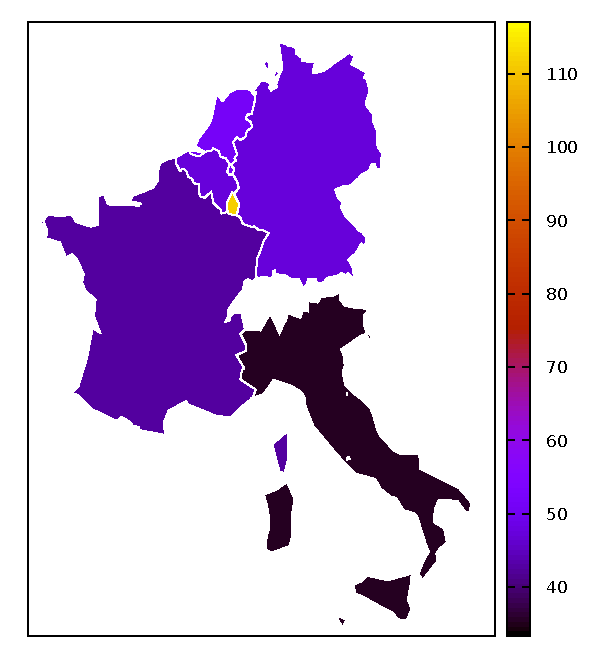
\includegraphics[scale=0.9]{GDPpc.pdf}
\end{center}
\caption{Output of script \texttt{founders.inp} (default gnuplot palette)}
\label{fig:founders}
\end{figure}


\section{Alignment problems}
\label{sec:pairing}

In order to produce a correct map it is essential that everything be
aligned properly: the map metadata, the payload series, and the
geometries of the regions. ``Region $i$'' must have the same referent
in all three contexts.

If the source map (GeoJSON or shapefile) is not broken we can assume
that the original metadata and the geometries are indeed aligned
correctly. But problems may arise (a) in aligning the payload and (b)
if one wishes to exclude some regions from the map. We discuss these
issues in turn.

\subsection{Aligning the payload}

In the somewhat unlikely case that the payload you wish to plot is
already included in the map metadata, no problem. But when the map
data and the payload come from different sources it may be tricky to
get them aligned properly. This problem is not specific to the mapping
apparatus---it's a more general issue concerning the matching of data
from different sources, addressed at length in the chapter titled
``Joining data sources'' in the \GUG{}---but it may be helpful to
offer a few comments here.

As mentioned above, the relevant tools provided by gretl are
\texttt{append} and \texttt{join}. A simple \texttt{append} will work
only if the regions appear in the same order in the map and payload
datasets. This is fairly easily checked if the number of regions is
small and each dataset contains readily comparable
identifiers. Otherwise---if the orders clearly differ or it's hard to
tell---it will be necessary to use \texttt{join}.

Look back at Listing~\ref{tab:founders-script}. In that case the map
and payload datasets contained the same set of two-letter identifiers
for the countries---albeit under different names, \texttt{FID} and
\texttt{code}---so \texttt{join} using the \option{ikey} and
\option{okey} options worked fine. In a different case, however, the
respective identifiers may not match up. For example, region names
might be in English in one dataset and in, say, Italian in the
other. Then you'll have to exercise your intelligence, but one idea is
to create an intermediate ``Rosetta stone'' file, maybe as CSV, giving
the mapping between the two identifiers, as in:
\begin{code}
# rosetta.csv
ID_en,ID_it
Apulia,Puglia
Sardinia,Sardegna
...
\end{code}
Then you can use \texttt{join} on the Rosetta file to add to the map
dataset the required identifier that's initially lacking.

\subsection{Sub-sampling}

In some cases one may wish to leave out certain outlying regions. For
example, it's quite common to produce thematic maps of the USA that
omit Hawaii, and perhaps Alaska. A related case is where the payload
value is missing (\texttt{NA}) for one or more regions.

In principle such cases threaten to break the required alignment of
payload and geometry, but in fact the \texttt{geomap} function handles
them, as follows.
\begin{itemize}
\item If the payload is \texttt{NA} for a given region, its geometry
  is automatically omitted from the map.
\item If the map dataset is sub-sampled, geometries corresponding
  to excluded observations are omitted.
\end{itemize}

The sub-sampling case is illustrated in Listing~\ref{tab:USA}: we use
the \texttt{smpl} command to cut out unwanted
regions. Figure~\ref{fig:USA} shows the results with and without
exclusion of Alaska and Hawaii.\footnote{Given the role of this
  example we don't bother adding a real payload, but just simulate
  data using the \texttt{normal} function.}

(\textbf{TODO}: In the case of missing payload values, we should
probably give the option of \textit{not} omitting the region, but
giving it a specific color representing ``missing data''.)

\begin{script}[p]
  \begin{scode}
open us-states.geojson --quiet --frompkg=geoplot
x = normal() # fake up some data!
opts = defbundle("plotfile", "us0.plt", "setpal", "blues")

# show the entire USA
opts.title = "USA (complete)"
geoplot($mapfile, x, opts)

# skip Alaska and Hawaii
smpl postal != "AK" && postal != "HI" --restrict
opts.title = "USA (mainland)"
opts.plotfile = "us1.plt"
geoplot($mapfile, x, opts)
  \end{scode}
  \caption{US maps, complete vs contiguous states}
  \label{tab:USA}
\end{script}

\begin{figure}[p]
  \begin{center}
  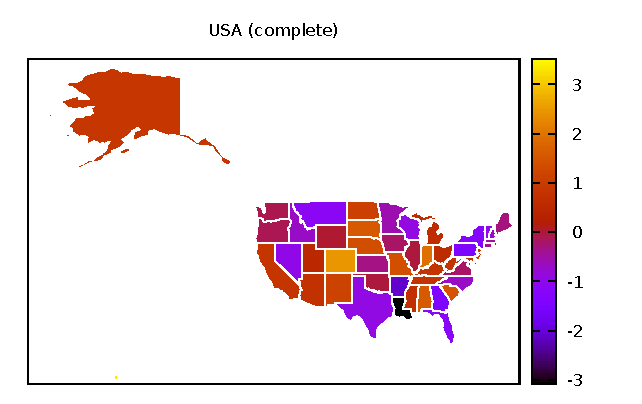
\includegraphics[scale=0.9]{us0.pdf}

  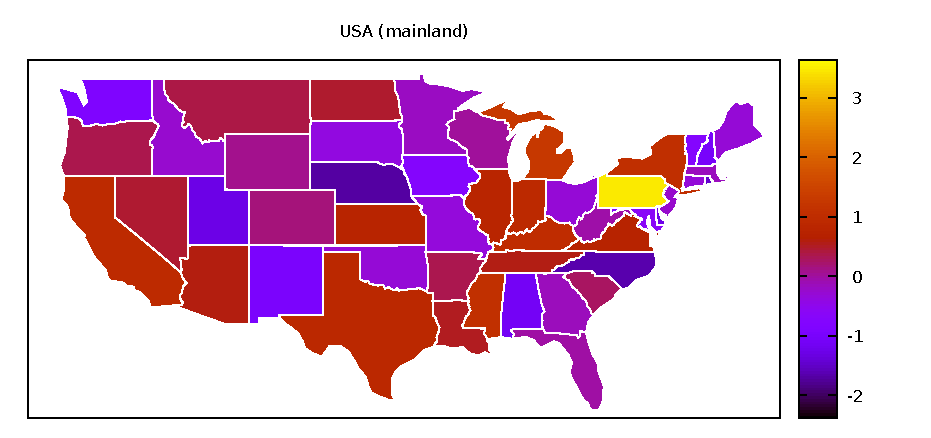
\includegraphics[scale=0.9]{us1.pdf}
\end{center}
\caption{Output of Listing \ref{tab:USA}}
\label{fig:USA}
\end{figure}

\section{Options for the \texttt{geoplot} function}
\label{sec:opts}

We first present all the currently supported options in alphabetical
order. Below the listing we give some further explanation of the usage
of \texttt{plotfile}, \texttt{show} and \texttt{inlined}.

\begin{description}
\item[\texttt{border}:] boolean, show a rectangular border around the
  map. Default: true. (FIXME maybe reverse the default?)
\item[\texttt{height}:] scalar, giving the height of the plot in
  pixels. Default: 600. Even if the desired output is a vector graphic
  (PDF or EPS) rather than a bitmap (see \texttt{plotfile} below),
  setting this value relative to the default can be used to adjust the
  size of the plot. For example \texttt{height = 400} will give a PDF
  graphic that's two-thirds of the default size.
\item[\texttt{inlined}:] boolean, to have the polygon data written
  directly into the \textsf{gnuplot} file. Default: false, the data
  are read from a separate file.
\item[\texttt{linecolor}:] string, naming the color in which to draw
  the borders of the regions. By default this is white if a payload is
  plotted, black if only outlines are shown.
\item[\texttt{linewidth}:] scalar, giving the width of the lines
  representing the borders of the regions. Setting this to 0
  suppresses those lines (unless no payload is supplied). Default:
  1.0.
\item[\texttt{literal}:] string containing \textsf{gnuplot} commands,
  for insertion before the actual \texttt{plot} command.
\item[\texttt{logscale}:] boolean, use log scale for the
  payload. Default: false.
\item[\texttt{plotfile}:] filename, allowing the user to direct
  output, either to a specified \textsf{gnuplot} command file or to a
  graphic file. If a command file is wanted the extension should be
  \texttt{plt}. If a graphic file is wanted you should give one of the
  following extensions: \texttt{png}, \texttt{pdf}, \texttt{eps},
  \texttt{emf} or \texttt{svg}.  If \texttt{plotfile} is given, but
  not as a full path, the file is written to the user's working
  directory.
\item[\texttt{projection}:] string, see~\ref{app:proj}.
\item[\texttt{palette}:] string, giving either a \textsf{gnuplot}
  \texttt{set palette} command or a predefined option, of which there
  are currently three: \texttt{blues}, \texttt{oranges} and
  \texttt{green-to-red}. For example, the syntax
  \begin{code}
    options.palette = "set palette defined (0 '#D4E4F2', 1 'steelblue')"
  \end{code}
  will give you a pleasing blue gradient---which also happens to be
  what you get by giving
  \begin{code}
    options.palette = "blues"
  \end{code}
  If no such string is given you get the default built-in
  \textsf{gnuplot} palette.
\item[\texttt{show}:] boolean, should the plot should be shown
  on-screen right away? Default: true. (Otherwise a file of some sort
  is written but not displayed---see \texttt{plotfile} above.)
\item[\texttt{tics}:] boolean, for turning on the printing of X
  (longitude) and Y (latitude) tics. Default: tics are suppressed,
  unless \texttt{geoplot} is invoked without any payload.
\item[\texttt{title}:] string specifying a title for the
  plot. Default: no title.
\end{description}

It may be helpful to run through various \texttt{geoplot} scenarios
with an eye to usage of the options.

\begin{enumerate}
\item You just want to see the map on-screen. Then don't give
  \texttt{plotfile} (or set it to \texttt{null}) and accept the
  default of \texttt{show} = 1.\label{just-see}
\item You want to see the map on-screen but also save the plot command
  file that generated it (maybe you want to edit the commands or pass
  them to \textsf{gnuplot} independently of gretl). Then specify
  \texttt{plotfile} with a \texttt{plt} extension.\label{see-and-save}
\item As in case 2 but you don't care to see the map on-screen: add
  \texttt{show} = 0.
\item You want to generate a graphic file (maybe for inclusion in a
  document or web page). Then give \texttt{plotfile} with one of the
  recognized graphic format extensions. In this case \texttt{show} is
  automatically turned off.
\end{enumerate}

Note that if you set \texttt{show} to 0 and do \textit{not} specify
\texttt{plotfile} that is tantamount to saying ``Don't do anything!'',
which is regarded as an error.

\subsection{Inlined data or not?}

As mentioned above, \texttt{geoplot} can pass the map coordinates to
\textsf{gnuplot} either by writing them directly into the plot command
file (\texttt{inlined} = 1), or by writing them to a separate data
file whose name is recorded in the command file (\texttt{inlined} =
0).

From the user's point of view, this distinction makes a difference
only if you're saving the plot command file (as in
scenario~\ref{just-see} or \ref{see-and-save} above).  In that
context, the advantage of having the data inlined is that, being all
in one file, the information required to generate a map cannot easily
become ``unstuck''. The disadvantage is that the command file may be
very large, and perhaps not so easy to edit; besides the actual
\textsf{gnuplot} commands it may contain many thousands of lines of
coordinates data (which in general \textit{should not be touched}, on
pain of breaking the map). At present we have \texttt{inlined} set to
0 by default but that may change; we recommend making an explicit
choice via the \texttt{options} bundle.

Note that if you specify \texttt{plotfile} as a \textsf{gnuplot}
command file, but not \texttt{inlined}, you'll get two output files:
the specified \texttt{plt} file plus a data file named by adding the
extension \texttt{dat}. For example you might get \texttt{mygeo.plt}
and \texttt{mygeo.plt.dat}, while with \texttt{inlined} = 1 you'd just
get a big \texttt{mygeo.plt}.

\section{Maps via the GUI}
\label{sec:gui}

To this point we have referred exclusively to executing commands and
calling functions. You can, of course, execute commands and call
functions in the GUI program via script or via the gretl console, but
what about point-and-click? Well, there is a certain amount you can do
in that way.

First, you can open a shapefile or GeoJSON file using the menu item
\textsf{/File/Open data/User file}. In the bottom right-hand corner of
the ``open file'' dialog, use the pull-down list to select
``Shapefiles'' or ``GeoJSON files''. You can also drag-and-drop such
files onto the main gretl window to the same effect.

Once map metadata are loaded in this way, the option \textsf{Display
  map} becomes available via the context (``right-click'') menu in the
main window, and also under \textsf{/View/Graph specified vars}. If
the current dataset contains one or more series that seem to gretl to
be plausible ``payload'' variables,\footnote{Admittedly, the heuristic
  employed for this purpose is not terribly clever.} invoking
\textsf{Display map} will produce a dialog box that allows you to
select one, in which case you'll get a choice of color palette to
represent it. Otherwise you just get to view the map outlines.

Further, the window shown by \textsf{Display map} offers a right-click
menu that allows saving the map (as PDF, EPS, PNG or EMF), copying
it to the clipboard, or saving it ``as an icon''.

So far, that's it. We may at some point expand the \textsf{Display
  map} dialog to offer more of the choices available via the
\texttt{options} argument to the \texttt{geoplot}
function. (\textbf{TODO}: even if we don't load up this dialog with
lots of options we should at least add a \textsf{Help} button which
gives a brief account of how to exploit more options via scripting.)

\section{``Expert'' refinements}
\label{sec:expert}

To recap, we have explained how map metadata can be brought in via the
\texttt{open} command (or via the GUI); how to add ``payload'' data;
and how to generate a map using the \texttt{geoplot} function. So far
so good, but that leaves open some questions that might occur to
ambitious users.  Can I open a map file, add a payload series, and
save a modified version of the map file including the payload? And in
relation to a map of the USA (for example), is there a way to include
Alaska and Hawaii, but ``tuck them underneath'' the continental US,
like I see in some graphics on the web?

Short answer: Yes. You can import a GeoJSON file (or shapefile) as a
gretl ``bundle'', using the \texttt{bread} function; make changes to
the bundle, then save it as GeoJSON using \texttt{bwrite}.

To get control over this it's necessary to understand the structure of
the bundle that \texttt{bread} produces when given map input. This
mimics the structure of a GeoJSON file (even if the input comes from a
shapefile), as shown in Listing~\ref{tab:geojson}; the labeling of
elements is as in GeoJSON, with gretl types in parentheses.

\begin{script}[htbp]
\begin{scode}
FeatureCollection (bundle)
  features (array of n bundles)
    features[i] (bundle)
      features[i].properties (bundle)
      features[i].geometry   (bundle)
        features[i].geometry.type (string)
        features[i].geometry.coordinates (array)
\end{scode}
  \caption{Structure of map data, gretl types in parentheses}
  \label{tab:geojson}
\end{script}

\subsection{Injecting payload data}
\label{sec:inject}

With this in mind, let's look at the relatively simple case of
injecting a payload series into a map file. Listing~\ref{tab:add-gdp}
revisits the EU founders map discussed in section~\ref{sec:example}.
As before, we start by opening the metadata and ``joining'' the GDP
per capita data. But now we open the GeoJSON as a bundle, and for each
\texttt{feature} (country) we augment its \texttt{properties} bundle
with the corresponding value of the \texttt{gdppc} series (under the
key ``\texttt{gdppc}''). Finally, we write the modified data to file.

\begin{script}[p]
\begin{scode}
open founders.geojson --quiet --frompkg=geoplot
join founders.csv gdp pop --ikey=FID --okey=code
series gdppc = 1000*gdp/pop

# open full GeoJSON as bundle
bundle b = bread($mapfile)

# add GDP per capita to properties
loop i=1..nelem(b.features)
   b.features[i].properties.gdppc = gdppc[i]
endloop

# save modified geojson file
bwrite(b, "founders_mod.json")
\end{scode}
  \caption{Adding payload data to a map file:
    \texttt{founders\_mod.inp}}
  \label{tab:add-gdp}
\end{script}

\subsection{Rearranging regions}
\label{sec:rearrange}

We now consider the case of rearranging regions of a given country (or
more generally, \texttt{features} within a given
\texttt{FeatureCollection}). Here we use the function
\texttt{geoplot\_translate\_feature}, which requires inclusion of
\texttt{geoplot.gfn} since it's not built in. Its signature is
\begin{code}
void geoplot_translate_feature(bundle *b, int f,
                               matrix shift,
                               matrix center[null],
                               matrix scale[null])
\end{code}
You pass in a map bundle obtained via \texttt{bread} (in pointer
form), the sequential index of the feature to translate, and a
2-vector \texttt{shift} giving displacement in the X and Y
directions. If in addition you want to rescale the feature you pass
two more 2-vectors: \texttt{center} holds the coordinates of the
feature's centroid and \texttt{scale} the scale factors to apply in
the two directions.

An example script is shown in Listing~\ref{tab:translate} and the
result of plotting the modifed GeoJSON file in
Figure~\ref{fig:usmod}. We obtain the second argument to pass to the
translator by inspection of the map dataset: Alaska is feature 48 and
Hawaii feature 5. In this case we decide to move Alaska 34$^{\circ}$
East and 35$^{\circ}$ South and shrink it substantially.  Getting the
effect one wants is likely to take some trial and error, but two
\textsf{geoplot} features can be helpful.

\begin{script}[p]
\begin{scode}
include geoplot.gfn

open us-states.geojson --quiet --frompkg=geoplot
bundle b = bread($mapfile)

# Shrink Alaska and place underneath the "lower 48"
matrix shift = {34, -35}
matrix center = {-150.885, 62.5503}
matrix scale = {0.3, 0.35}
geoplot_translate_feature(&b, 48, shift, center, scale)

# Shift Hawaii alongside Alaska
shift = {51, 5}
geoplot_translate_feature(&b, 5, shift)

# save modified geojson file
bwrite(b, "us_modified.json")
\end{scode}
  \caption{Moving Alaska and Hawaii}
  \label{tab:translate}
\end{script}

\begin{figure}[p]
  \centering
  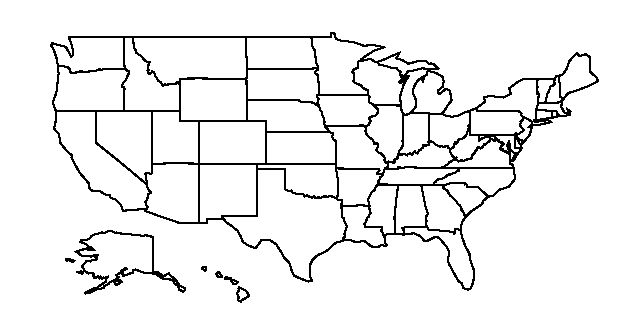
\includegraphics{usmod.pdf}
  \caption{Alaska and Hawaii moved}
  \label{fig:usmod}
\end{figure}

First, if you plot just the map outlines (no payload) then you should
see the X and Y values on the axes, giving you at least a rough idea
of the shifts you might want. Second, \textsf{geoplot} contains the
function \texttt{geoplot\_describe\_json} which gives you a good deal
of relevant information. This signature of this function is
\begin{code}
bundle geoplot_describe_json (const bundle jb, int verbose[1])
\end{code}
You pass a map bundle and a verbosity level, as in
\begin{code}
include geoplot.gfn
bundle us = bread("us-states.geojson")
geoplot_describe_json(us, 3)
\end{code}
On searching the \texttt{verbose} = 3 output for Alaska one finds
(here's a small snippet):
\begin{code}
  48: geometry type = MultiPolygon, no id
        ...
        name: Alaska
        ...
        Extents: X = {-171.791,-129.98}; Y = {54.4042,70.6964}
\end{code}
The \texttt{Extents} data enable you to figure out plausible
values for the \texttt{center} of a feature.

\section{Future directions?}
\label{sec:future}

We've alluded at various points above to possible extensions of
\textsf{geoplot}. Here we collect various ideas---no promises, though!

\begin{itemize}
\item The \texttt{geoplot} function could be complemented with a
  ``command block'' variant, on the pattern of the existing gretl
  \texttt{plot} block. Some users might find this sort of interface
  more comprehensible and convenient.
\item We could provide a more fully featured graphical interface for
  selection of options that inflect the appearance of maps.
\item Besides just colorizing map polygons, we might add support
  for showing geographical features such cities, roads or rivers.
  And/or labeling of regions.
\item An ambitious project for the longer term could be adding support
  for TopoJSON, an extension of GeoJSON that encodes topology. See
  \url{https://github.com/topojson/topojson}.
\end{itemize}

\section*{Coda}

In the foregoing we have mostly kept things simple with toy
examples. In concluding, we'll show off with a ``real'' example:
Figure~\ref{fig:ita-covid} shows the distribution of COVID cases
across Italian provinces as of 2020-05-15. The appearance of this plot
was tuned using the following option settings:
\begin{code}
string cmds = sprintf("set colorbox user origin 0.9,0.45 size 0.03,0.4\n")
cmds ~= sprintf("set xrange [6.4:20.5]")
bundle opts = defbundle("plotfile", "covid.pdf")
opts.logscale = 1
opts.border = 0
opts.linewidth = 0.4
opts.setpal = "green-to-red"
opts.literal = cmds
opts.height = 900
\end{code}

As you'll have seen in the previous figures, the default
\textsf{gnuplot} ``colorbox'' is quite large, occupying the full
height of the plot.  This doesn't look so great for a tall, skinny
country like Italy, so we used the \texttt{literal} option to pass in
commands to make the colorbox smaller and reposition it; to prevent it
from going off the right edge of the plot we also made the
\texttt{xrange} a little wider than the default. We were able to
determine what the revised \texttt{xrange} should look like by
examining a plot with no payload, showing the values on the axes.

\begin{figure}[p]
  \centering
  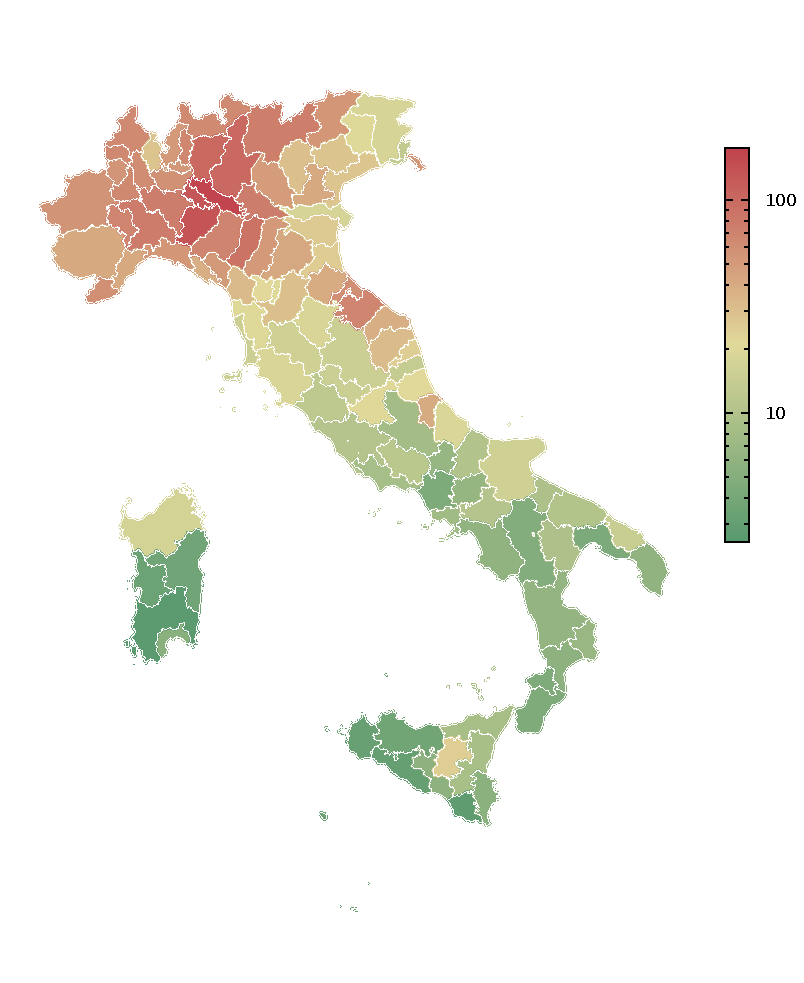
\includegraphics{covid.pdf}
  \caption{COVID-19 cases per 10\,000 by province as of
    2020-05-15, log scale}
  \label{fig:ita-covid}
\end{figure}


\clearpage
\startappendices

\myappendix{Representation of polygons in gnuplot}
\label{sec:gnuplot}

The
following \textsf{gnuplot} code
\begin{code}
  unset key
  plot '-' using 1:2:3 with filledcurves fillcolor "blue"
  0 0 0
  0.5 0 0.866
  1 0 0
  e
\end{code}
produces an equilateral triangle: 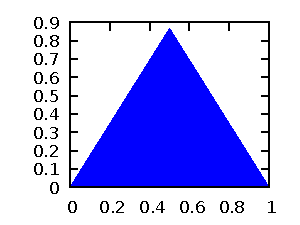
\includegraphics[height=2cm]{triangle.pdf}

\medskip

The internal coloring of polygons can be set using ``\texttt{fillcolor
  palette}''. For example,
\begin{code}
unset key
$coords << EOD
0 0 2.5
0 1 2.5
1 1 2.5
1 0 2.5

2 1 3.5
2 2 3.5
3 2 3.5
3 1 3.5

4 0 3
4 1 3
5 1 3
5 0 3
EOD
plot for [i=0:*] $coords index i with filledcurves fillcolor palette
\end{code}
(where the third column of the data indexes into the palette) produces
\begin{center}
  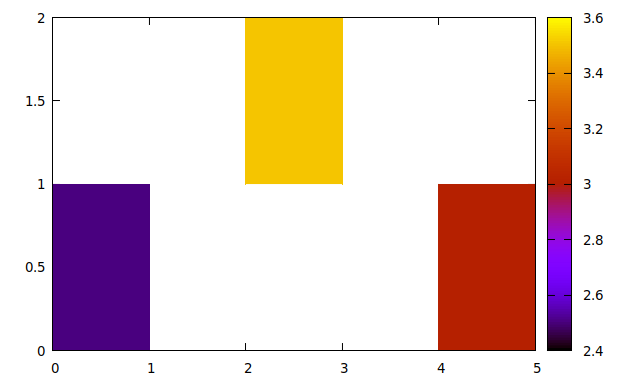
\includegraphics[width=0.6\textwidth]{squares}
\end{center}

A nice way to customize the palette is via ``\texttt{set
  palette defined}'' (see the \textsf{gnuplot} manual; also see
section~\ref{sec:opts} above).

\clearpage
\myappendix{Projections}
\label{app:proj}

\textsf{Geoplot} assumes (mostly, but see below) that incoming map
coordinates are given as degrees of latitude (Y) and longtitude
(X). This is mandated by RFC 7946, which has governed GeoJSON since
2016; it also appears to be the most common case for ESRI shapefiles.

Everyone knows that the Earth is not actually a sphere, but let's
assume it is for simplicity. Then a degree of latitude is always the
same length on the ground: 1/360 of the planet's circumference. But
the length of a degree of longitude varies, from 1/360 of Earth's
circumference at the equator to zero at the poles. So imagine that we
pass the X--Y pairs to our plotting engine on the assumption that ``a
degree'' is always the same size: the result will be more or less OK
close to the equator but at higher or lower latitudes features will be
seriously stretched horizontally (or squashed vertically) relative to
what we're used to seeing. To avoid this effect some sort of
projection is required.

By default geoplot uses what we might call a ``quasi-Mercator''
projection. In most cases this should produce maps that look quite
acceptable and it has the advantage of simplicity. All we do is take
the height of the plot as specified by the user (or a default of 600
pixels) and figure out what the width should be to make a degree of
longitude the same size as a degree of latitude at the mid-point
latitude. However, we offer four alternatives, as follows:
\begin{center}
  \begin{tabular}{cll}
    EPSG id & description & option string \\[4pt]
  \textsf{3857} & standard Mercator & \verb|"Mercator"| \\
  \textsf{4326} & ``null'' projection & \verb|"EPSG4326"| \\
  \textsf{2163} & U.S. National Atlas Equal Area &
     \verb|"EPSG2163"| \\
  \textsf{3035} & Europe Equal Area & \verb|"EPSG3035"|
\end{tabular}
\end{center}

Figure~\ref{fig:proj} compares the available projections for the
contiguous United States. In this case the default \textsf{geoplot}
projection and standard Mercator are practically
indistinguishable. \textsf{EPSG:4326}, which treats degrees as
everywhere the same size, exhibits the horizontal stretching mentioned
above. \textsf{EPSG:2163} gives the impression of looking at the USA
on a section of the globe.

\begin{figure}[htbp]
  \centering
  \begin{tabular}{cc}
    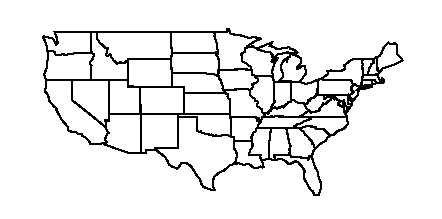
\includegraphics[scale=0.9]{prj0.pdf} &
     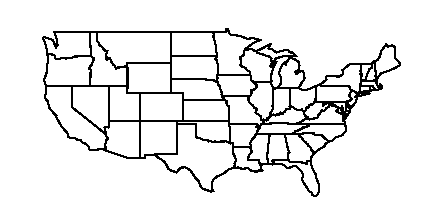
\includegraphics[scale=0.9]{mercator.pdf} \\[-6pt]
    \small{Default} & \small{Mercator} \\
    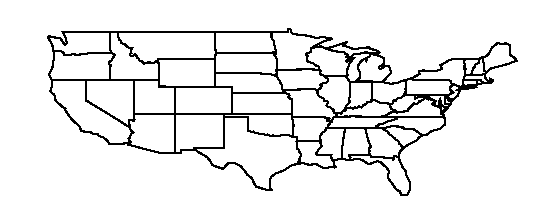
\includegraphics[scale=0.9]{epsg4326.pdf} &
      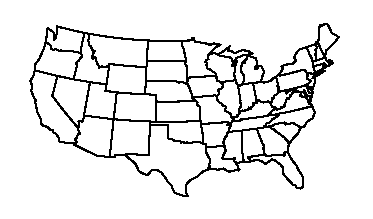
\includegraphics[scale=0.9]{epsg2163.pdf} \\[-6pt]
    \small{EPSG:4326} & \small{EPSG:2163}
  \end{tabular}
  \vspace{1ex}
  \caption{Comparison of projections}
  \label{fig:proj}
\end{figure}

To select one of the alternatives, you add the appropriate string to
the \texttt{options} bundle passed to the \texttt{geoplot} function
under the key \texttt{projection}. Please note that \textsf{EPSG:2163}
is specially tuned for the USA, and will produce weird-looking or
non-existent results for other parts of the world. \textsf{EPSG:3035}
is similarly tuned for Europe. They are both so-called Lambert
Azimuthal Equal Area projections.

\subsection*{Non-standard coordinates}

In certain map files---maybe GeoJSON predating RFC 7946, and perhaps
some shapefiles---the X--Y coordinates are not in the expected form of
degrees of latitude and longitude. In that case they probably already
encode some sort of projection, and so should not be ``re-projected''.
For GeoJSON files, \textsf{geoplot} makes an attempt to determine
whether a non-standard coordinate system is used, as was allowed under
the obsolete GeoJSON 2008 specification. In that case we automatically
cancel projection; we also do this if the X or Y values are out of
bounds for representing degrees (that is, |X| > 180 or |Y| > 90).

Failing such automatic detection, one can try specifying
\textsf{EPSG:4326} to get the X and Y units to be treated as equal in
size, in effect cancelling projection, as in
\begin{code}
bundle options
options.projection = "EPSG4326"
\end{code}

For anyone wishing to follow up on this sort of thing, there are many
websites presenting information on coordinate systems and
projections. Two of the most useful ones, in our experience, are:

Reference materials: \url{https://spatialreference.org/}

Explanation:
\url{https://source.opennews.org/articles/choosing-right-map-projection/}

\clearpage
\myappendix{Specialized functions}
\label{app:special}

The functions shown below are implemented in hansl and included in the
\textsf{geoplot} addon; to use them you must first do
\begin{verbatim}
include geoplot.gfn
\end{verbatim}

\begin{funcdoc}
\begin{verbatim}
bundle geoplot_describe_json (const bundle jb, int verbose[1])
\end{verbatim}
  Provides a systematic description of the GeoJSON bundle \texttt{jb},
  the amount of detail depending on the \texttt{verbose} setting,
  which has a maximum of 3. By assigning the return value one can
  obtain a bundle containing the information but for some purposes the
  printed output may suffice. See section~\ref{sec:rearrange}.
\end{funcdoc}

\begin{funcdoc}
\begin{verbatim}
void geoplot_set_properties (bundle *b, list L)
\end{verbatim}
  Rewrites the \texttt{properties} within the bundle representation of
  a map, \texttt{b}, to include all and only the series referenced in
  the list \texttt{L}. Provides a means of adding ``payload'' data
  (see section~\ref{sec:payload}) and also pruning unwanted metadata.
  In the example below, \texttt{us-states.geojson} originally contains
  40 items of metadata per state, most of them unlikely to be of
  interest.
\begin{code}
# example
open us-states.geojson --quiet --frompkg=geoplot
join statepop.gdt population --ikey=postal --okey=Code

# select only the properties we actually want
list L = name postal population
bundle b = bread($mapfile)
geoplot_set_properties(&b, L)
bwrite(b, "us_pruned.json")
\end{code}
\end{funcdoc}

\begin{funcdoc}
\begin{verbatim}
function void geoplot_translate_feature (bundle *b, int f,
                                         matrix shift,
                                         matrix center[null],
                                         matrix scale[null])
\end{verbatim}
  Shifts the feature with sequential index \texttt{f}, optionally
  rescaling it. See~\ref{sec:rearrange} for an example and
  explanation.
\end{funcdoc}

\begin{funcdoc}
\begin{verbatim}
function matrix geoplot_seek_feature(const bundle b,
                                     string name,
                                     bool do_plot[1])
\end{verbatim}
  Searches the map bundle \texttt{b} for features matching
  \texttt{name} (on a case-insensitive basis). If one or more matches
  are found their 1-based indices are returned in a row vector.  If a
  single match is found metadata for the feature are printed and if
  \texttt{do\_plot} is not set to zero a plot of the feature is
  shown.
\begin{code}
include geoplot.gfn
open us-states.geojson --frompkg=geoplot --quiet
map = bread($mapfile)
# no matches
geoplot_seek_feature(map, "nowhere")
# two matches
geoplot_seek_feature(map, "CAROLINA")
# one match, plot shown
geoplot_seek_feature(map, "Florida")
\end{code}
\end{funcdoc}

\begin{funcdoc}
\begin{verbatim}
function void geoplot_simplify(bundle *b,
                               scalar preserve[0.1:1:0.75])
\end{verbatim}
  Simplifies the polygons in the map bundle \texttt{b} using
  Visvalingam's algorithm. This may be useful if for a certain
  geography of interest the only map file readily available is at a
  higher resolution than you need. Smaller values of the
  \texttt{preserve} parameter preserve less detail or in other words
  simplify the map more radically; the default value of 0.75 may be
  considered conservative if you start with a very detailed map.
\begin{code}
include geoplot.gfn
open highres.geojson --quiet
bundle map = bread($mapfile)
geoplot_simplify(&map, 0.5)
bwrite(map, "simplified.geojson")
open simplified.geojson --quiet
# see if the level of detail is OK
geoplot($mapfile)
\end{code}
\end{funcdoc}

\end{document}

%%% Local Variables:
%%% mode: latex
%%% TeX-master: t
%%% End:
